\lecture{Auth Network \& ISO/OSI}{30~-~01~-~2026}
%
%
\section{Fondamenti dell'autenticazione}
L'autenticazione è il processo fondamentale per verificare l'identità in un sistema digitale. Possiamo distinguere due tipologie principali:
\begin{itemize}
    \item \textbf{Peer Authentication}: Verifica l'identità dell'interlocutore con cui si sta comunicando;
    \item \textbf{Data Authentication}: Verifica la provenienza e l'integrità dei dati ricevuti.
\end{itemize}

Per autenticarsi, ci si basa su tre categorie di fattori, spesso combinati tra loro:
\begin{enumerate}
    \item \emph{Something that you know}: Qualcosa che conosci (es. una password);
    \item \emph{Something that you are}: Qualcosa che sei (es. dati biometrici);
    \item \emph{Something that you have}: Qualcosa che possiedi (es. un token o uno smartphone).
\end{enumerate}

%
\subsection{Protocollo di Autenticazione}
Il processo tipico avviene tramite uno scambio di messaggi (challenge-response): Alice invia il suo ID a Bob chiedendo un servizio. Bob risponde con una richiesta di prova (challenge). Alice invia la prova (es. la password o un digest crittografico). Se la prova è valida, l'autenticazione ha successo.
Vedi grafico \ref{graph:auth}.

\begin{figure}
    \centering
    \begin{tikzpicture}[
            node distance=5cm,
            font=\sffamily,
            >=Stealth, % Stile delle frecce
            actor/.style={
                    draw,
                    rectangle,
                    rounded corners,
                    minimum width=2.5cm,
                    minimum height=1cm,
                    fill=blue!10,
                    thick,
                    align=center
                },
            msg/.style={
                    ->,
                    thick,
                    shorten >=2pt,
                    shorten <=2pt
                },
            txt/.style={
                    midway,
                    above,
                    font=\small,
                    align=center
                },
            note/.style={
                    draw=gray,
                    dashed,
                    fill=yellow!10,
                    font=\scriptsize,
                    align=left,
                    inner sep=5pt
                }
        ]

        % --- 1. Definizione degli Attori ---
        \node[actor] (Alice) {Alice\\(Utente)};
        \node[actor, right=of Alice] (Bob) {Bob\\(Servizio/Server)};

        % --- 2. Linee Temporali ---
        % Coordinate finali per le linee
        \coordinate[below=7cm of Alice] (EndAlice);
        \coordinate[below=7cm of Bob] (EndBob);

        % Disegno le linee verticali
        \draw[thick, gray] (Alice.south) -- (EndAlice);
        \draw[thick, gray] (Bob.south) -- (EndBob);

        % --- 3. Scambio Messaggi ---

        % Step 1: Alice invia ID
        \draw[msg, blue] ($(Alice.south)+(0,-1)$) -- node[txt] {1. Inizio conversazione\\(Richiesta Servizio)} ($(Bob.south)+(0,-1)$);

        % Step 2: Bob invia Challenge
        \draw[msg, red] ($(Bob.south)+(0,-2.5)$) -- node[txt] {2. Challenge\\(Richiesta di Autenticazione)} ($(Alice.south)+(0,-2.5)$);

        % Nota facoltativa: Alice calcola la prova
        \node[note, anchor=east] at ($(Alice.south)+(-0.5,-5.5)$) {Alice invia la sua\\prova univoca};

        % Step 3: Alice invia Proof
        \draw[msg, blue] ($(Alice.south)+(0,-4)$) -- node[txt] {3. Risposta autenticazione\\(Alice ID)} ($(Bob.south)+(0,-4)$);

        % Step 4
        \draw[msg, red] ($(Bob.south)+(0,-5.5)$) -- node[txt] {4. Challenge \\(Richiesta di prova, es. password \dots)} ($(Alice.south)+(0,-5.5)$);

        % Step 4: Verifica e Successo
        \node[note, anchor=west] at ($(Bob.south)+(0.5,-7)$) {Bob verifica la prova:\\\textbf{Se valida $\rightarrow$ OK}};

        \draw[msg, green!60!black, dashed] ($(Alice.south)+(0,-7)$) -- node[txt] {5. Prova inviata\\(Auth riuscita)} ($(Bob.south)+(0,-7)$);

    \end{tikzpicture}
    \caption{}\label{graph:auth}
\end{figure}


In contesti sicuri, non si invia mai la password in chiaro, ma si utilizzano \emph{algoritmi di digest} (hashing):
\begin{itemize}
    \item \textbf{Chiave Simmetrica}: Entrambi i dispositivi (A e B) condividono una chiave segreta (sym key). Si calcola il digest del messaggio combinato con la chiave. Se i digest calcolati da entrambi coincidono, l'identità è verificata.
    \item \textbf{Crittografia Asimmetrica (Firma Digitale)}: Si utilizza una coppia di chiavi. Il mittente cripta il digest del messaggio con la propria chiave privata (firma digitale). Il ricevente decifra il digest con la chiave pubblica del mittente e lo confronta con quello calcolato localmente. Se corrispondono, l'origine è autenticata.
\end{itemize}

%
\section{Architettura di rete}
La comunicazione tra dispositivi è estremamente complessa. Per renderla gestibile, utilizziamo i \emph{protocolli di comunicazione}, che danno significato alle sequenze di bit e gestiscono esigenze specifiche come l'instradamento (routing) o l'affidabilità.
Per organizzare questi protocolli, adottiamo un \emph{Modello a Strati (Layer Model)}. Ogni protocollo appartiene a uno specifico livello in base alla sua funzionalità.

%
\subsection{Vantaggi del Modello a Strati}
È cruciale per l'esame comprendere perché usiamo questo modello:
\begin{itemize}
    \item \textbf{Modularità e Indipendenza}: Ogni livello svolge un compito preciso ed è indipendente dagli altri.
    \item \textbf{Astrazione}: I livelli superiori si occupano delle applicazioni, quelli inferiori dei dettagli tecnici della trasmissione, semplificando lo sviluppo software.
    \item \textbf{Scalabilità}: Si possono aggiungere nuovi protocolli senza modificare le parti esistenti.
    \item \textbf{Interoperabilità}: Standardizza il linguaggio, permettendo a dispositivi di produttori diversi di comunicare.
\end{itemize}
%
\subsection{ISO/OSI vs TCP/IP}
Esistono due modelli di riferimento principali:
\begin{enumerate}
    \item \textbf{Modello ISO/OSI (7 Livelli)}: Fisico, Data Link, Network, Trasporto, Sessione, Presentazione, Applicazione.
    \item \textbf{Modello TCP/IP (4 Livelli)}: Link, Internet, Trasporto, Applicazione.
\end{enumerate}
\begin{note*}
    Il livello Applicazione del TCP/IP accorpa i livelli dell'ISO/OSI dentro altri, vedi figura \ref{fig:stacked}.
    \begin{figure}
        \centering
        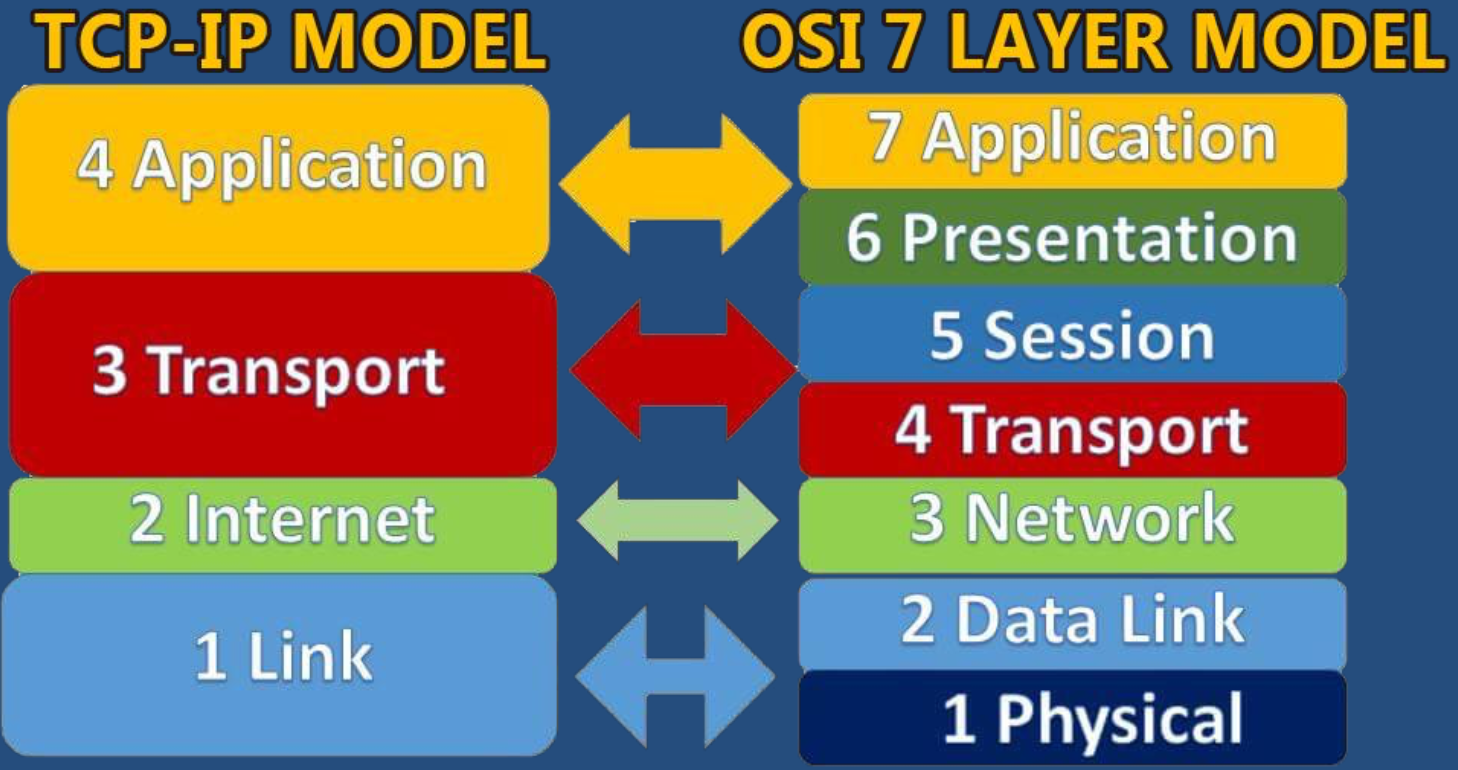
\includegraphics[width=0.7\linewidth]{assets/Screenshot 2026-01-31 at 15.04.43.png}
        \caption{TCP/IP e ISO/OSI}\label{fig:stacked}
    \end{figure}
\end{note*}

%
\subsubsection{Analisi livelli}
%
\paragraph{Layer 1: Physical} Si occupa della trasmissione grezza dei bit attraverso un mezzo fisico (cavi, fibra, onde radio).
\begin{itemize}
    \item \textbf{Funzione}: Codifica i dati digitali in segnali e gestisce la sincronizzazione tra mittente e ricevente (clock);
    \item \textbf{PDU (Protocol Data Unit)}: Bit.
\end{itemize}

%
\paragraph{Layer 2: Data-link}
Fornisce un collegamento affidabile tra due nodi direttamente connessi.
\begin{itemize}
    \item \textbf{Funzione}: Organizza i bit in ``frame'', gestisce l'indirizzamento fisico (\emph{MAC Address}) e il controllo degli errori a livello locale;
    \item \textbf{PDU}: Frame.
\end{itemize}

%
\paragraph{Layer 3: Network}
Gestisce l'instradamento (routing) dei dati tra reti diverse e remote.
\begin{itemize}
    \item \textbf{Funzione}: Utilizza indirizzi logici (Indirizzi IP) per identificare i dispositivi e determinare il percorso migliore (path) attraverso i router;
    \item \textbf{PDU}: Pacchetti (packet).
\end{itemize}

%
\paragraph{Layer 4: Transport}
Gestisce la comunicazione ``end-to-end'' creando un canale logico tra le applicazioni.
\begin{itemize}
    \item \textbf{Funzione}: Utilizza le \emph{Porte} (es. TCP o UDP ports) per indirizzare i dati alla giusta applicazione (\emph{Multiplexing}). Può garantire affidabilità, correzione errori e controllo di flusso;
    \item \textbf{Protocolli principali}: TCP (affidabile, orientato alla connessione) e UDP.
    \item \textbf{PDU}: Segmento.
\end{itemize}

%
\paragraph{Layer 5: Session}
Stabilisce, gestisce e termina le sessioni di comunicazione (es. una comunicazione complessa che include una invio e ricevimento continuo in modo correlato).

%
\paragraph{Layer 6: Presentation}
Stabilisce e converte i dati in un formato appropriato, in modo che entrambe le parti possano comprenderli (formattazione dati, codifica, compressione \dots).

%
\paragraph{Layer 7: Application}
È l'interfaccia con l'utente e il software. Include protocolli come HTTP (web), SMTP (email), FTP (file).

%
\subsubsection{Incapsulamento e PDU}
Ogni livello aggiunge le proprie informazioni di controllo (Header) ai dati ricevuti dal livello superiore. Questo processo è detto incapsulamento. Una PDU (anche chiamata \emph{Transmission Unit}) è composta da Header + Payload (i dati veri e propri).
Ogni livello tratta l'intero pacchetto del livello superiore come semplice ``payload'' da trasportare. Vedi figura \ref{fig:ppdu}.

\begin{figure}
    \centering
    \begin{subfigure}{0.45\linewidth}
        \centering
        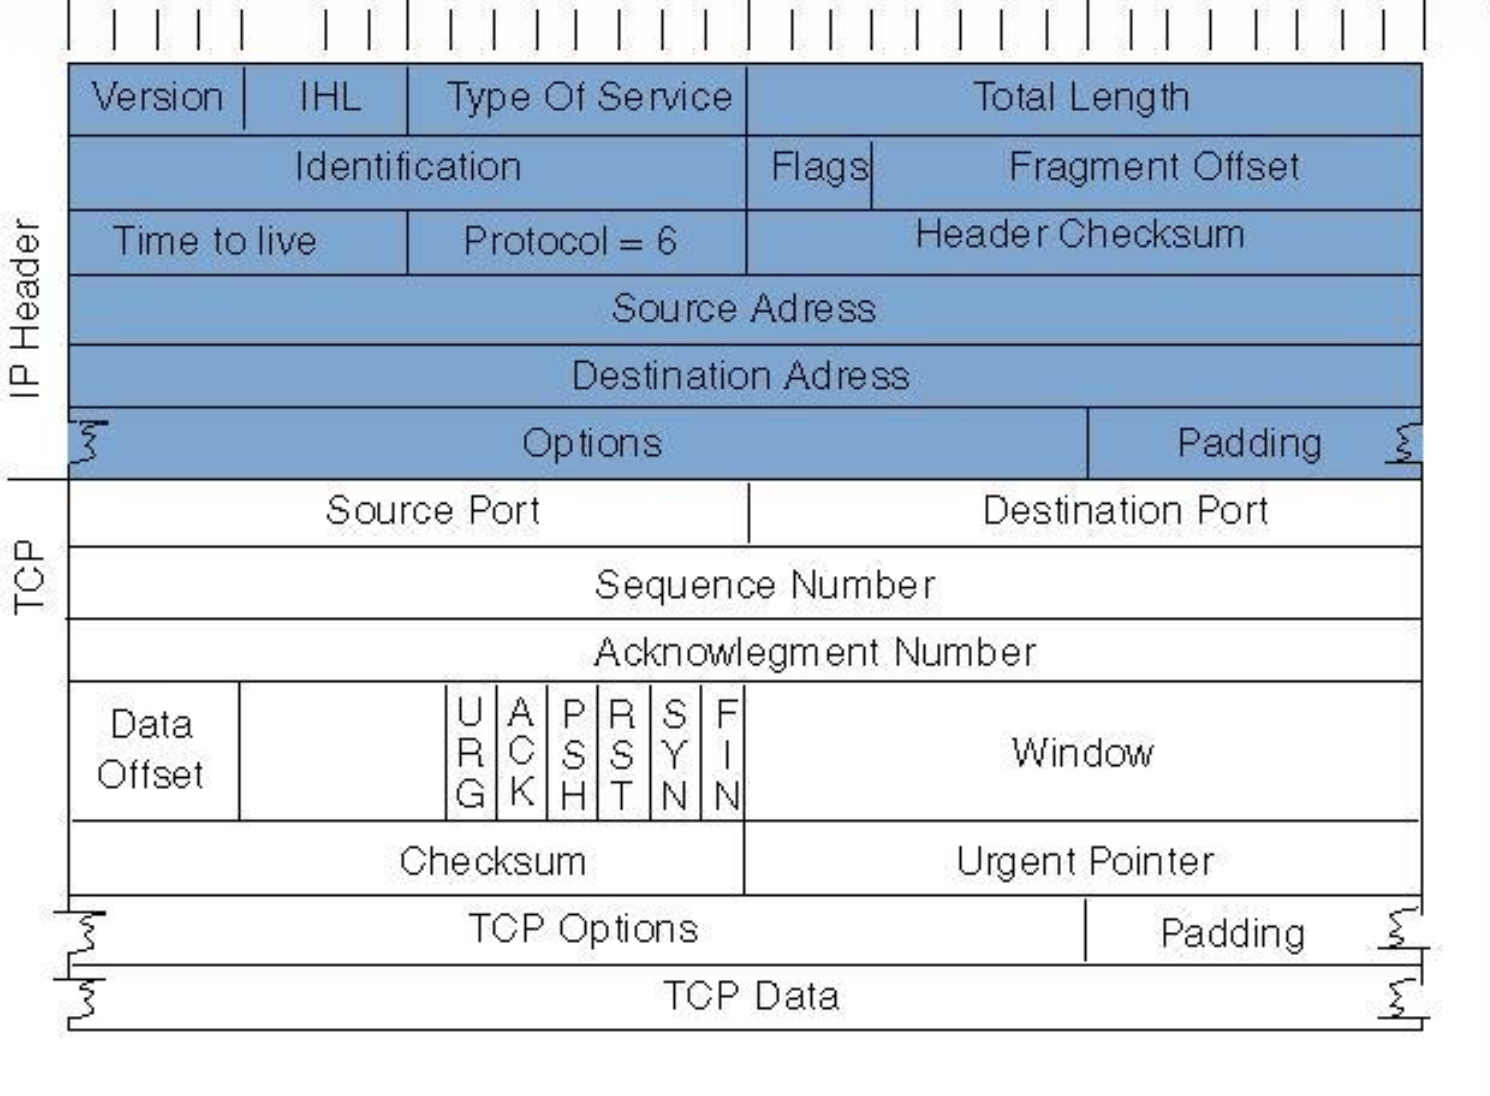
\includegraphics[width=\linewidth]{assets/Screenshot 2026-01-31 at 15.30.33.png}
        \caption{Packet Header}\label{fig:head}
    \end{subfigure}
    \begin{subfigure}{0.45\linewidth}
        \centering
        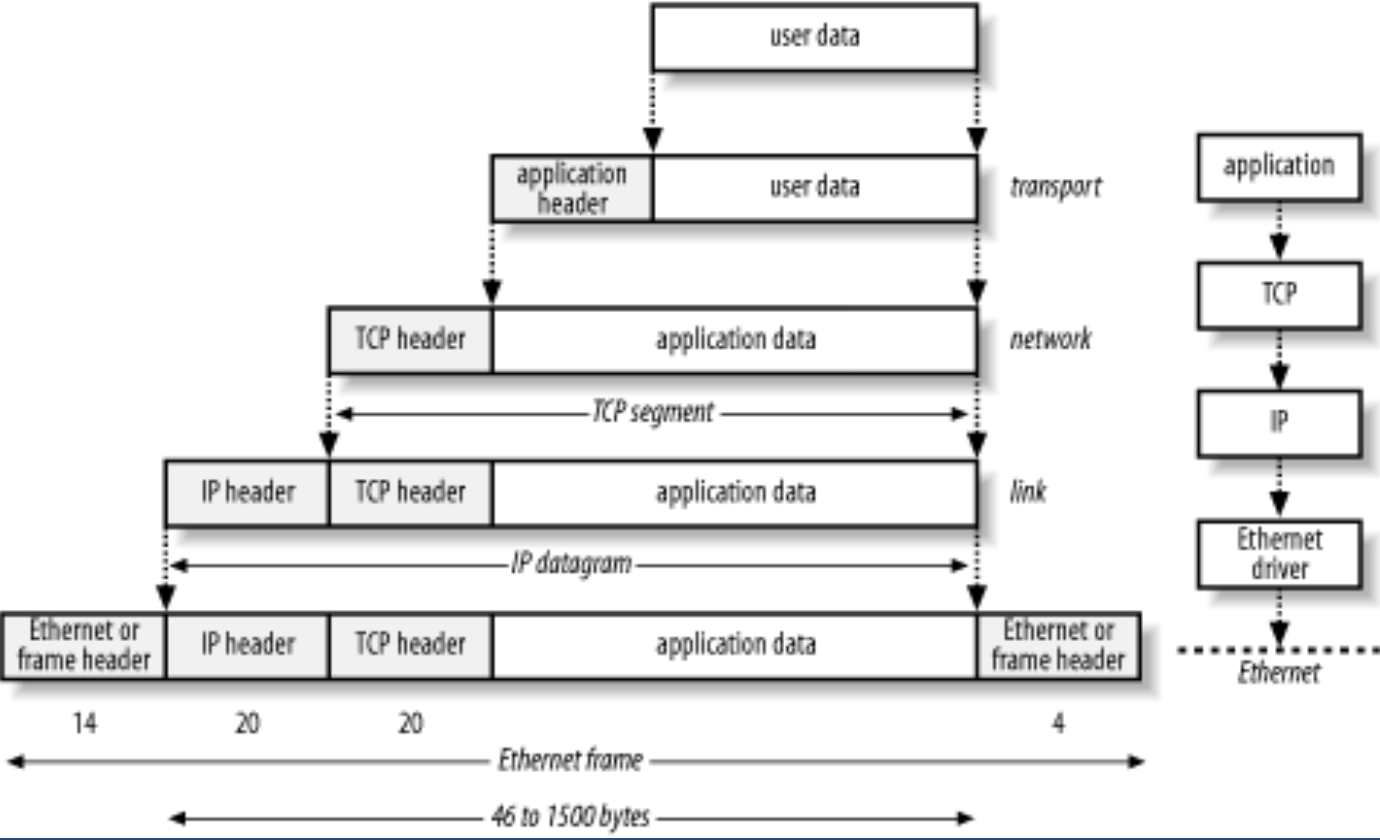
\includegraphics[width=\linewidth]{assets/Screenshot 2026-01-31 at 15.30.49.png}
        \caption{PDU Flow}\label{fig:flow}
    \end{subfigure}
    \caption{Pacchetti e PDU}\label{fig:ppdu}
\end{figure}

%
\section{Meccanismi di rete}
%
\subsection{TCP Handshake}
Il protocollo TCP stabilisce una connessione affidabile tramite il ``Three-Way Handshake'':
\begin{itemize}
    \item \textbf{SYN}: Il client chiede di connettersi ($ \text{seq}=x $);
    \item \textbf{SYN-ACK}: Il server risponde confermando ($ \text{ack}=x+1 $) e proponendo la sua sequenza ($ \text{seq}=y $);
    \item \textbf{ACK}: Il client conferma la ricezione ($\text{ack} = y+1 $).
\end{itemize}
Vedi figura \ref{fig:handshake}.

\begin{figure}
    \centering
    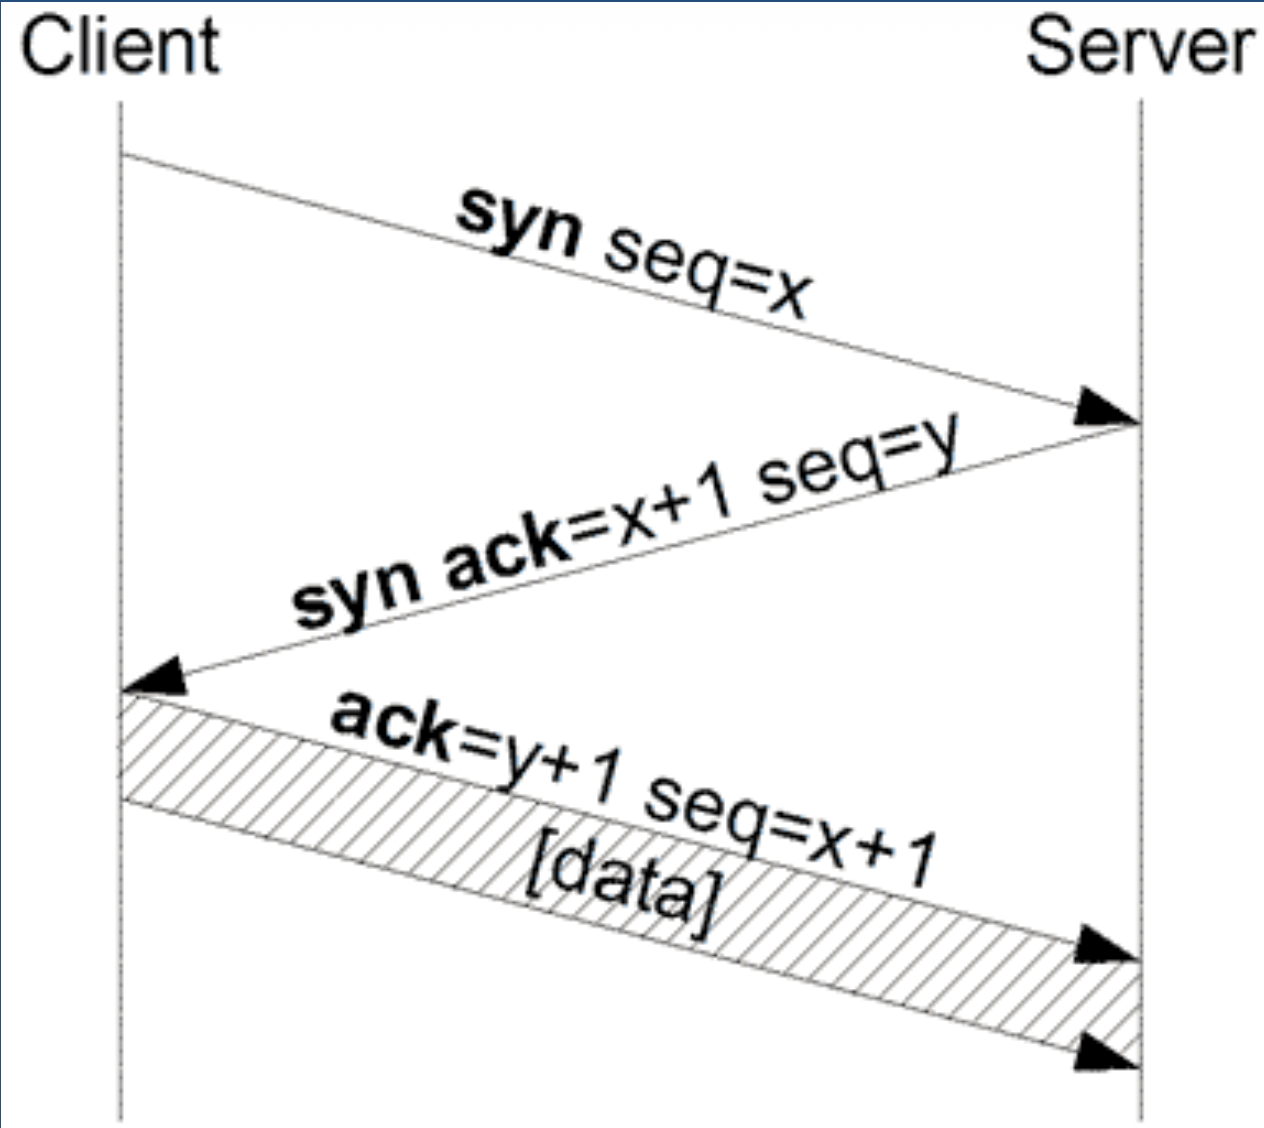
\includegraphics[width=0.5\linewidth]{assets/Screenshot 2026-01-31 at 15.35.41.png}
    \caption{TCP Handshake}\label{fig:handshake}
\end{figure}

%
\subsection{Routing e DNS}
Nel \textbf{Routing} i pacchetti viaggiano attraverso molteplici ``hop'' (salti) tra router per raggiungere la destinazione.

Il \textbf{DNS} (Domain Name System) è la ``rubrica'' di Internet. Traduce i nomi di dominio leggibili (es. \lstinline|www.google.it|) in indirizzi IP numerici necessari alla rete. Se un server DNS non conosce l'IP, interroga altri server e poi salva il risultato in cache.

%
\subsection{Strumenti di analisi di rete}
Per interagire con la rete e fare diagnosi, utilizziamo specifici strumenti:
\begin{itemize}
    \item \emph{Ping}: Verifica se un host è raggiungibile e misura il tempo di risposta (latenza);
    \item \emph{Traceroute}: Mostra tutti i passaggi intermedi (hop) che i dati fanno per arrivare a destinazione;
    \item \emph{Netstat}: Analizza le connessioni attive e le statistiche;
    \item \emph{Nslookup}: Interroga il DNS per risolvere nomi in IP;
    \item \emph{Wireshark}: Uno strumento visuale avanzato per catturare e analizzare nel dettaglio ogni singolo pacchetto di traffico (protocolli, header, payload). Vedi figura \ref{fig:wireshark}.
\end{itemize}

\begin{figure}
    \centering
    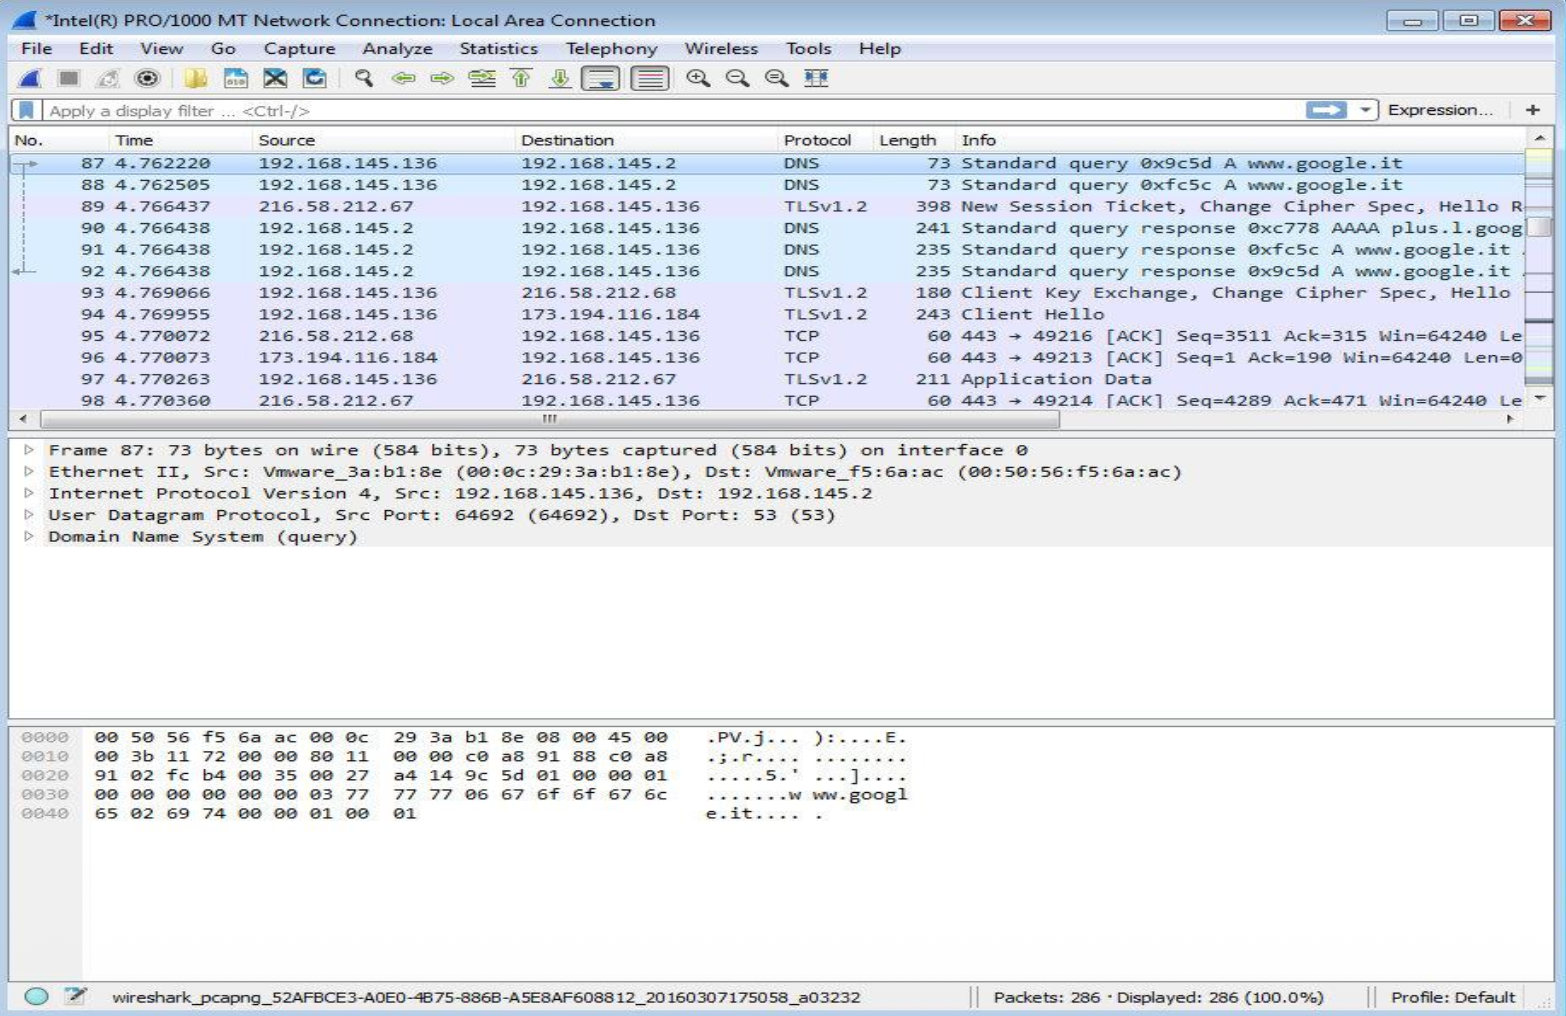
\includegraphics[width=0.6\linewidth]{assets/Screenshot 2026-01-31 at 15.43.51.png}
    \caption{Wireshark}\label{fig:wireshark}
\end{figure}